\chapter{Les ondes stationnaires}
Lorsqu'une impulsion unique, une onde simple, est envoyée sur une corde fixée à ses deux extrémités, elle va se réfléchir et revenir \enquote{inversée} c'est-à-dire avec la même élongation, mais une vitesse opposée. Si, au lieu d'une onde unique, on envoie une onde continue (voir \ref{Onde unique et onde entretenue}), les ondes réfléchies vont interférer avec les ondes directes et l'ensemble va présenter un profil complexe.

Toutefois, si la fréquence est choisie de manière adéquate par rapport à la vitesse de l'onde et la longueur de la corde, il est possible de créer une \motcle{onde stationnaire} : une situation dans laquelle les ondes réfléchies interfèrent constructivement avec les ondes directes à certains endroits et destructivement à d'autres.


Les points d'interférence destructive, qui sont donc immobiles sont appelés \motcle{noeuds}. Les points d'interférence constructive sont appelés \motcle{anti-noeuds} ou \motcle{ventres}.
La plus petite fréquence permettant d'obtenir une onde stationnaire donne un profil tel qu'illustré ci-dessous :

\begin{figure}[ht!]
    \centering
    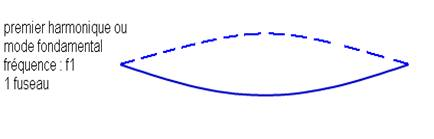
\includegraphics[width=.8\linewidth]{onde_stationnaire_fond1.png}
    \caption{Mode fondamentale d'une onde stationnaire : un ventre, deux n\oe{}ds.}
\end{figure}

Le profil de l'onde correspond à : \(L=\frac{\lambda}{2}\) où L est la longueur de la corde. La fréquence associée est : \(f=\frac{v}{2 \cdot L}\). Cette première onde stationnaire est appelée \motcle{première harmonique} ou \motcle{fondamentale}.

La deuxième fréquence permettant d'obtenir une onde stationnaire donne le profil ci-dessous :
\begin{figure}[ht!]
    \centering
    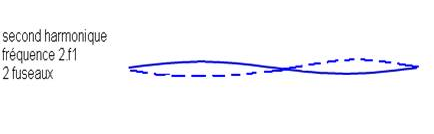
\includegraphics[width=.8\linewidth]{onde_stationnaire_harm2.png}
    \caption{Deuxième harmonique : deux ventres, trois n\oe{}ds.}
\end{figure}

Le profil de l'onde correspond à : \(L=2 \cdot \frac{\lambda}{2}\). La fréquence associée est : \(f=\frac{v}{ L}\). Cette deuxième onde stationnaire est appelée \motcle{deuxième harmonique}.

La troisième harmonique est associée au profil ci-dessous, pour lequel  \(L=3 \cdot \frac{\lambda}{2}\).
\begin{figure}[ht!]
    \centering
    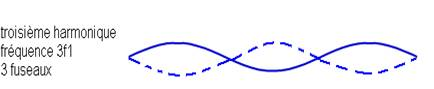
\includegraphics[width=.8\linewidth]{onde_stationnaire_harm3.png}
    \caption{Troisième harmonique : trois ventres, quatre n\oe{}ds.}
\end{figure}

Si on généralise, on voit que les différentes ondes stationnaires qui peuvent prendre place sur une corde de longueur \(L\) avec les deux extrémités fixes correspondent à  \(L=k \cdot \frac{\lambda}{2}\) et que les fréquences associées valent :
\begin{equation}
    f=k \cdot \frac{v}{2 \cdot L}
\end{equation}

Au cours de la séance de labo sur les ondes stationnaires, nous avons vu que la vitesse d'une onde sur une corde dépend de la tension dans la corde, \(F_T\), et de la masse linéique, \(\mu\). La relation utilisée était : \(v=\sqrt{\frac{F_T}{\mu}}\). Si on combine les deux relations, on constate que les fréquences permettant l'obtention d'une onde stationnaire sur une corde soumise à une tension \(F_T\) et d'une masse linéique \(\mu\) s'obtiennent par :
\begin{equation}
    f=k \cdot \sqrt{\frac{F_T}{4\cdot \mu \cdot L^2}}
\end{equation}

Selon la valeur de \(k\), on obtient la première, la deuxième, la troisième, \ldots harmonique.

\newpage

\section{Application : instrument à corde}
Lorsqu'on pince une corde de guitare, des ondes de fréquences très variées sont générées. La plupart de ces ondes disparaissent rapidement, mais les ondes stationnaires persistent. Il n'y a pas qu'une harmonique qui persiste, mais une combinaison de différentes harmoniques.

La longueur de la corde est fixée par celle du manche (distance entre le point d'attache et l'extrémité du manche), les clés permettent de régler la tension et le type de corde détermine la masse linéique.
Lorsque le joueur produit un \(La\), la corde vibre simultanément à différentes harmoniques.

Puisque la corde est fixée à ses deux extrémités, les harmoniques sont des multiples entiers les unes des autres : 220, 440, 660, \ldots [Hz]. C'est la proportion des différentes harmoniques qui constitue le son propre, le \motcle{timbre}, du \(La\) sur une  guitare et qui le distingue de la même note sur un autre instrument.

\begin{figure}[ht!]
    \centering
    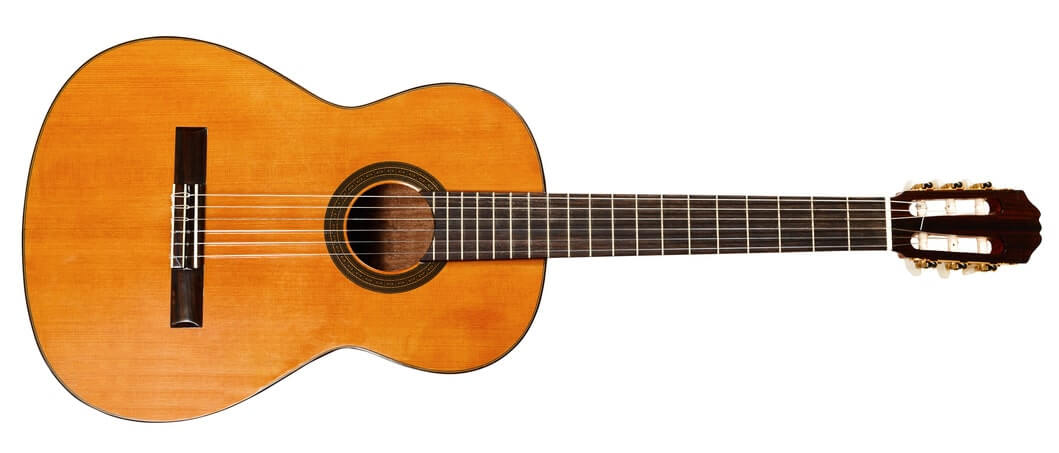
\includegraphics[width=.5\linewidth]{guitare.png}
    \caption{Une guitare}
\end{figure}

\newpage

\begin{figure}[ht!]
    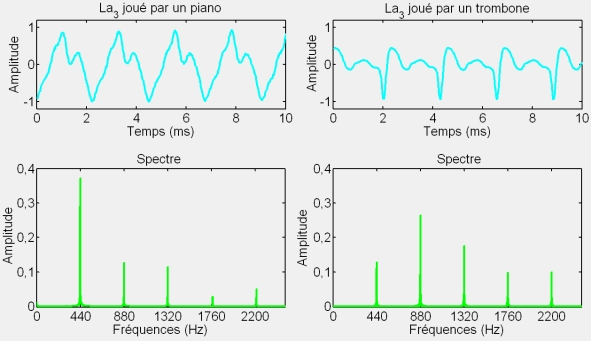
\includegraphics[width=.8\linewidth]{spectre_sonore.png}
    \caption{Le spectre sonore d'un trombone et d'un piano pour la note La. C'est le spectre qui détermine le timbre.}
\end{figure}

\begin{figure}[ht!]
    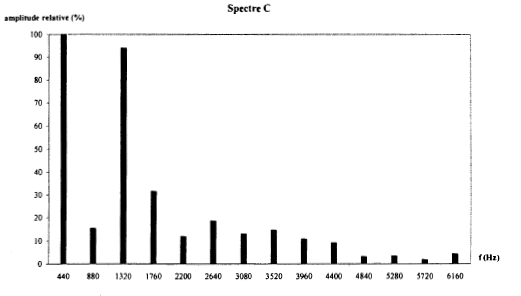
\includegraphics[width=.8\linewidth]{spectre_guitare_la.png}
    \caption{Le spectre d'une guitare pour la note La}
\end{figure}

\newpage

\section{Exercices}
\begin{exercise}
    La longueur et la masse d'une corde de piano sont respectivement de 1,1m et de 9,00 g.
    \begin{enumerate}[a)]
        \item Quelle doit être la tension dans la corde pour qu'elle vibre à une fréquence fondamentale de 131 Hz (Do, octave 3) ?
        \item Quelles sont les fréquences des quatre premières harmoniques ?
    \end{enumerate}
\end{exercise}
\begin{solution}
    \(F_T=679,58[N]\)
\end{solution}

\begin{exercise}
    Un ukulélé \enquote{concert} a une longueur de corde d'environ 40cm, tandis qu'une guitare à une longueur de 64cm. On souhaite produire la même fondamentale sur ces deux instruments. Si on place la même corde sur les deux instruments, laquelle doit être la plus \enquote{tendue} ? Quel est le rapport entre les deux tensions ?
    \begin{figure}[ht!]
        \centering
        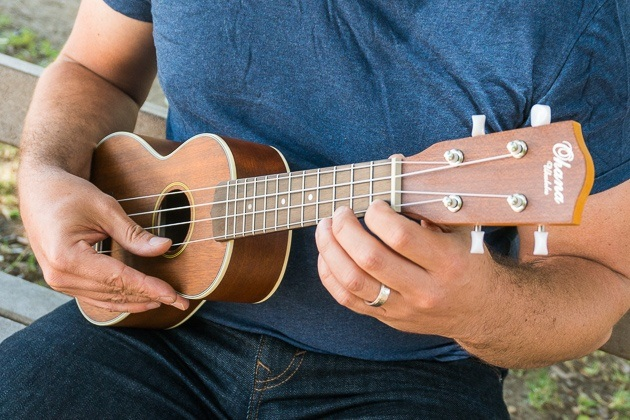
\includegraphics[width=.4\linewidth]{ukulele.png}
        \caption{Un ukulélé}
    \end{figure}
\end{exercise}
\begin{solution}
    Dans cette situation, \(\mu\) est identique pour les deux instruments puisqu'il s'agit de la même corde. Donc :
    \(\frac{F_{T1}}{L_1 ^2}=\frac{F_{T2}}{L_2 ^2}\) \\
    Si on remplace \(L_1\) et \(L_2\) par leurs valeurs respectives, on obtient :\\
    \(F_{T1}=0,3906 \cdot F_{T2}\) .\\
    \(F_{T1}\) est donc plus petit que \(F_{T2}\), la deuxième corde est plus tendue que la première. Le rapport entre les deux tensions est de \(0,3906\).
\end{solution}


\begin{exercise}
    Une corde de violon vibre à 440[Hz] lorsqu'on la relâche après l'avoir pincée. À quelle fréquence vibre-t-elle si on la pince après avoir diminué sa longueur de 25\% ?
\end{exercise}
\newpage
\begin{solution}
    \begin{equation*}
        \begin{aligned}
            f_1                   & =\sqrt{\frac{F_T}{4 \mu L_1 ^2}}                                               \\
            f_2                   & =\sqrt{\frac{F_T}{4 \mu (0,75 L_1)^2}}                                         \\
            \frac{f_1}{f_2}       & =\frac{\sqrt{\frac{F_T}{4 \mu L_1 ^2}}}{\sqrt{\frac{F_T}{4 \mu (0,75 L_1)^2}}} \\
            \frac{f_1 ^2}{f_2 ^2} & =\frac{F_T}{4 \mu L_1 ^2}  \cdot \frac{4 \mu (0,75 L_1)^2}{F_T}                \\
            \frac{f_1}{f_2}       & =\frac{3}{4}                                                                   \\
            f_2                   & =\frac{4}{3} \cdot f_1                                                         \\
            f_2                   & =586,67[Hz]
        \end{aligned}
    \end{equation*}

\end{solution}

\begin{exercise}
    La vitesse des ondes sur une corde de 5,496 [m] est de 480 m/s. Un régime stationnaire est obtenu si la fréquence est de 131[Hz].
    \begin{enumerate}[a)]
        \item Combien de noeuds y'a-t-il ?
        \item À quelle distance les uns des autres se trouvent les noeuds ?
    \end{enumerate}
\end{exercise}
\begin{solution}
    \begin{enumerate}[a)]
        \item Il y a 4 noeuds.
        \item La distance entre deux noeuds est de \(\frac{\lambda}{2}\), donc : \(d=1,8321[m]\)
    \end{enumerate}
\end{solution}

\begin{exercise}
    On attache une corde horizontale d'une masse linéique de \(4,2 \times 10^{-4} [kg \cdot m^{-1}]\) par l'une de ses extrémités à un vibrateur oscillant à 60[Hz] avec une faible amplitude. La corde passe par une poulie située à une distance \(L=1,4[m]\) de l'extrémité fixée au vibrateur et des poids sont suspendus à l'autre extrémité.
    Quelle doit être la masse suspendue à l'extrémité de la corde pour produire 5 ventres ? On considère que l'extrémité fixée au vibrateur correspond à un noeud, car l'amplitude du signal est faible par rapport à celle des interférences.
\end{exercise}
\begin{solution}
    On sait que : \(F_T=\frac{f^2 \cdot 4 \cdot \mu \cdot L^2}{k^2}\). \\
    Dans cette situation, \(k=5\) puisqu'on veut obtenir 5 ventres. Donc :\\
    \(F_T=0,4742[N]\) \\
    \(m=0,04833[kg]\)

\end{solution}